\subsection{Necessidade de Desenho de Software Resiliente}
Grande parte dos sistemas contemporâneos são sistemas distribuídos, ou seja, representam um conjunto de computadores independentes entre si, ligados através de uma rede de dados, que se apresentam aos utilizadores como um sistema único e coerente~\cite{fcc-distributed-systems}.
No entanto, essa interdependência traz consigo o risco de falhas, e quando um desses componentes falha, toda ou parte da funcionalidade do sistema pode ser comprometida.
Tal pode resultar em perda de dados, indisponibilidade de serviços e outros problemas, dependendo da criticidade do(s) componente(s) afetado(s)~\cite{cap-theorem}.
É neste contexto que surge a necessidade de desenhar software resiliente, capaz de lidar com falhas e manter a sua funcionalidade mesmo quando um ou mais dos seus componentes falham ou estão temporariamente indisponíveis.

% \subsection{Tolerância a Falhas vs. Resiliência}

\subsection{Bibliotecas como Mecanismos de Resiliência}
Fornecem mecanismos para lidar com as eventuais falhas inerentes a componentes de um sistema distribuído, tentando garantir ao máximo a
disponibilidade e confiabilidade dos serviços que estes disponibilizam.

\begin{table}[h]
    \centering
    \label{tab:resilience_libraries}
    \begin{tabular}{|l|l|l|}
        \hline
        \textbf{Biblioteca}                      & \textbf{Linguagem} & \textbf{Plataforma} \\ \hline
        Netflix's Hystrix~\cite{netflix-hystrix} & Java               & JVM                 \\ \hline
        Resilience4j~\cite{resilience4j}         & Java/Kotlin        & JVM                 \\ \hline
        Polly~\cite{polly-dotnet}                & C\#                & .NET                \\ \hline
    \end{tabular}
    \caption{Exemplos de bibliotecas como mecanismos de resiliência}
\end{table}

Exemplos de mecanismos de resiliência disponibilizados por estas bibliotecas:

\begin{itemize}[topsep=0pt,itemsep=0pt,partopsep=0pt, parsep=0pt]
    \item \textbf{Retry}: Tenta novamente uma operação que falhou, aumentando a probabilidade de sucesso;
    \item \textbf{Rate Limiter}: Limita a taxa de requisições que um serviço pode receber;
    \item \textbf{Circuit Breaker}: Interrompe, temporariamente, a comunicação com um serviço que está a falhar, de forma a evitar que o mesmo sobrecarregue o sistema. Semelhante a um disjuntor elétrico;
    \item \textbf{Fallback}: Fornecer um valor ou executa uma ação alternativa caso uma operação falhe.
\end{itemize}

A biblioteca Polly~\cite{polly-dotnet} divide os mecanismos de resiliência que disponibiliza em duas categorias:

\begin{itemize}[topsep=0pt,itemsep=0pt,partopsep=0pt, parsep=0pt]
    \item \textbf{Resiliência Reativa}: Reage a falhas e mitiga o seu impacto;
    \item \textbf{Resiliência Proativa}: Previne que as falhas aconteçam.
\end{itemize}

De referir que, as bibliotecas mencionadas anteriormente serão exploradas ao longo da fase de planeamento e desenvolvimento do projeto, de forma a que se possa tirar proveito do conhecimento inerente à sua implementação.
Com especial atenção para a biblioteca \textit{Resilience4j}~\cite{resilience4j}, uma vez que apresenta um módulo de interoperabilidade com \textit{Kotlin} para a plataforma \textit{JVM}.

\subsection{Kotlin Multiplatform}

A tecnologia \textif{Kotlin Multiplatform}~\cite{kmp} possibilita a partilha do código nativo da aplicação entre diversas plataformas, tornando-o independente de qualquer plataforma específica.

Para cada plataforma alvo, regularmente denominada como \textit{target}, poderão ter que existir implementações adicionais porque:

\begin{itemize}[topsep=0pt,itemsep=0pt,partopsep=0pt, parsep=0pt]
    \item Um determinado \textit{target} não suporta diretamente o \textit{KMP}, como é o caso do \textit{Node.js}, e por isso é necessário criar um \textit{adapter} para a comunicação com o código comum (\textit{CommonMain} - que está em \textit{Kotlin});
    \item Uma determinada funcionalidade não consegue ser implementada de forma comum porque:
    \begin{itemize}[topsep=0pt,itemsep=0pt,partopsep=0pt, parsep=0pt]
        \item é necessário saber detalhes específicos do \textit{target} para a sua implementação.
        Usando o padrão \textit{expect/actual} é possível criar definições comuns (\textit{expect}) e implementações específicas para cada \textit{target} (\textit{actual});
        \item as bibliotecas disponíveis para código comum (\textit{Standard Kotlin Library + Kotlinx}) não cobrem a(s) funcionalidade(s) pretendida(s) e não ser que se utilize outra(s) biblioteca(s) \textit{KMP} como dependência(s) do projeto, se existir(em).
    \end{itemize}
\end{itemize}

\begin{figure}[H]
    \centering
    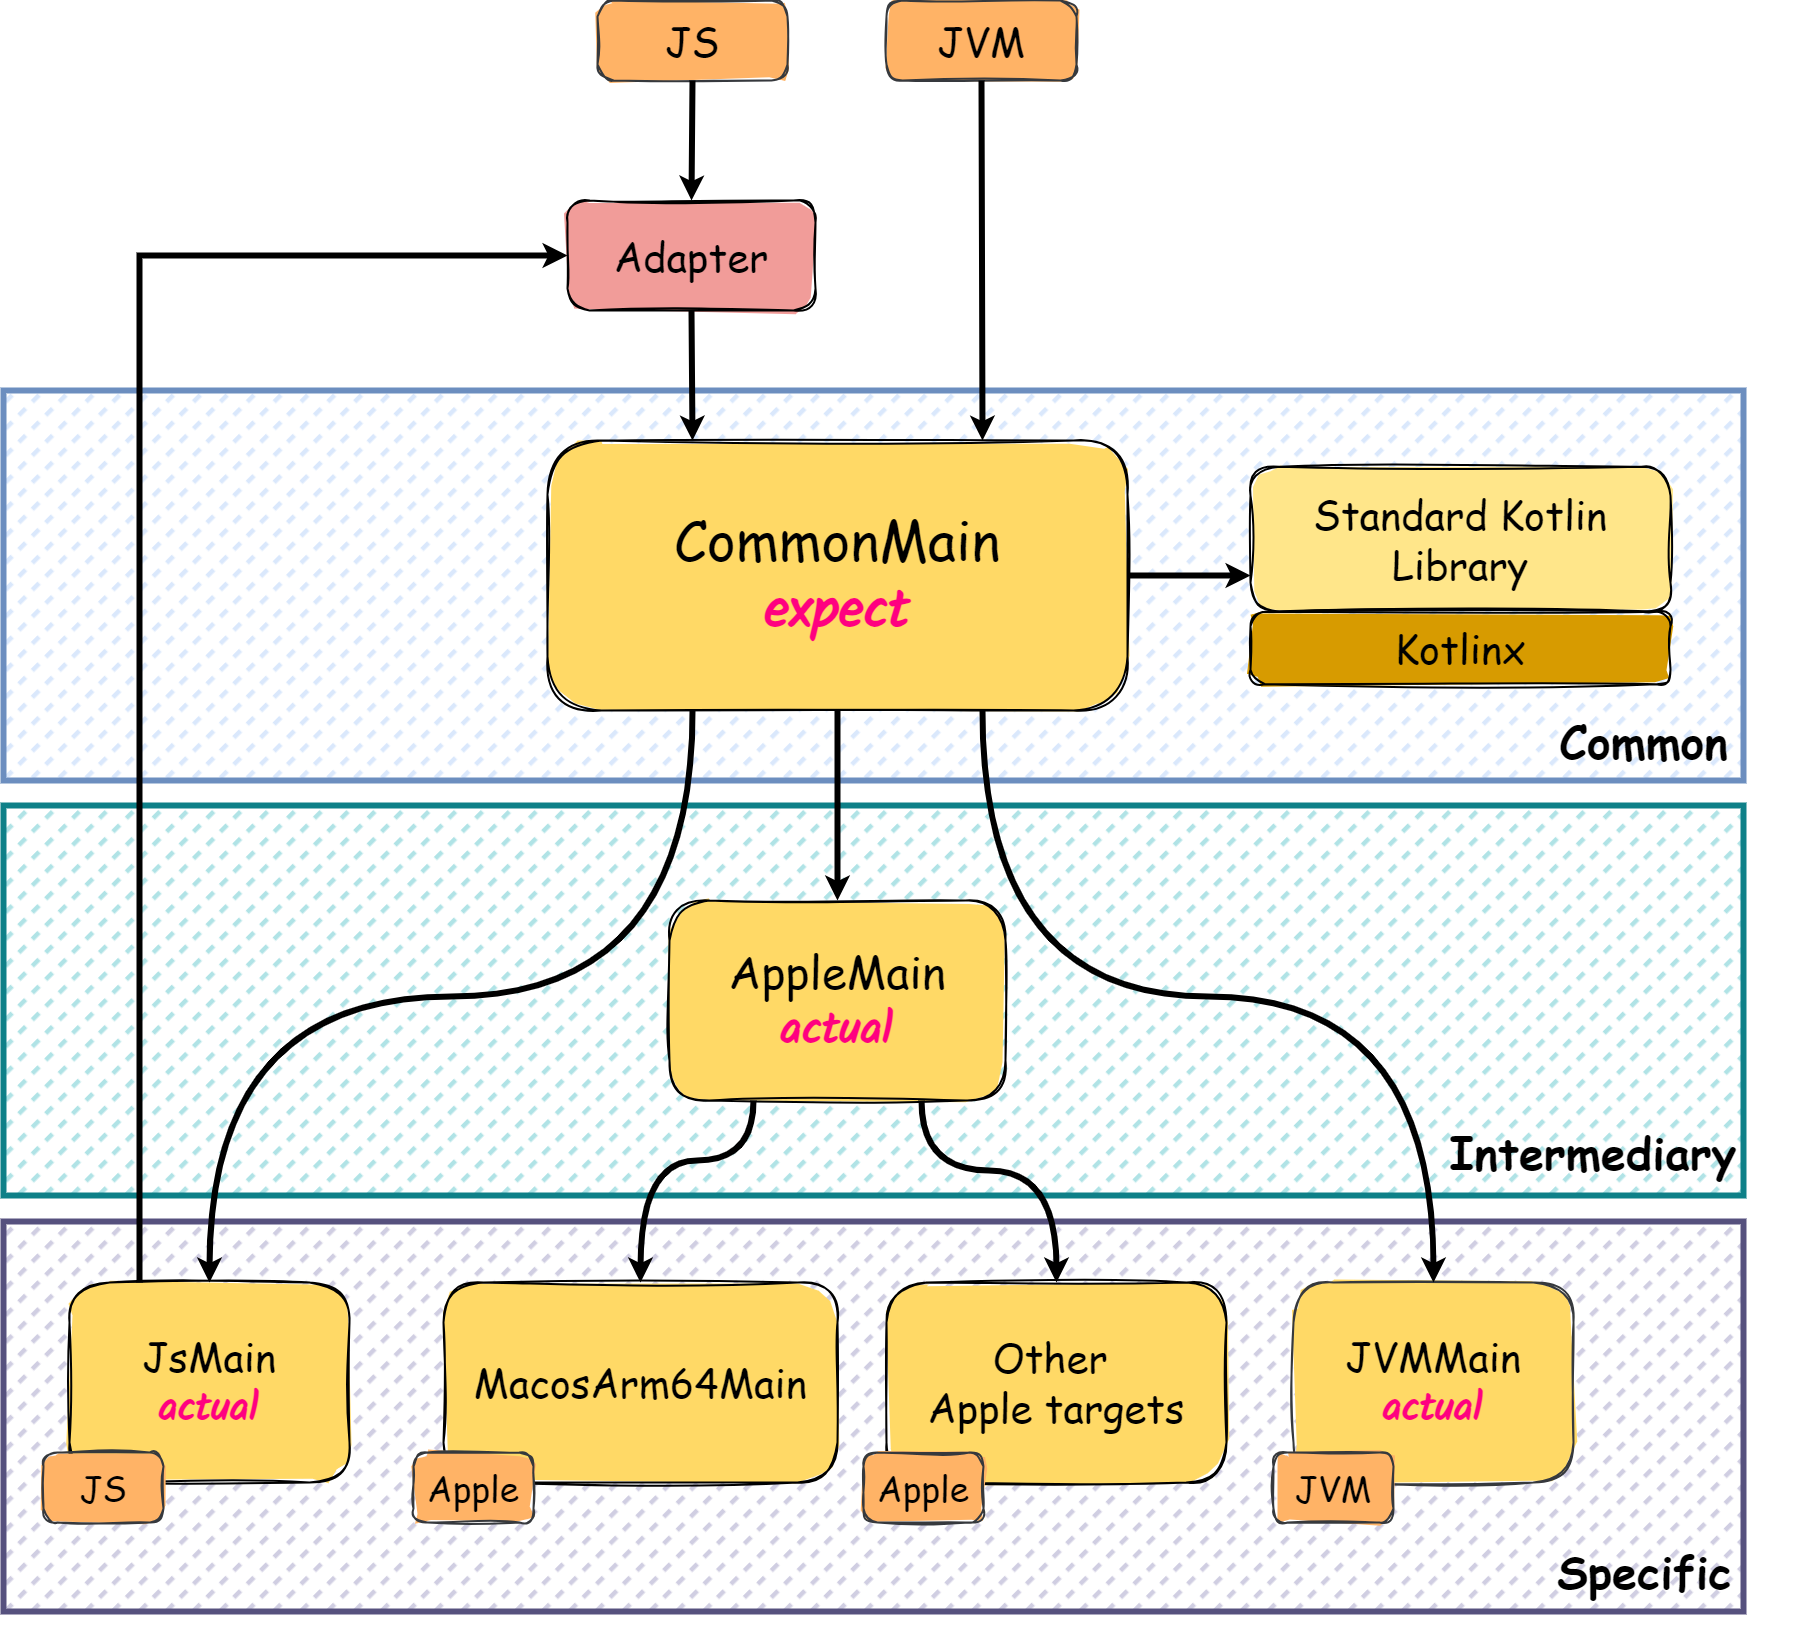
\includegraphics[width=0.5\textwidth]{../docs/imgs/kmp-architecture}
    \caption{Arquitetura do KMP}
    \label{fig:kmp-architecture}
\end{figure}

Portanto, o objetivo principal do \textit{KMP} é maximizar a reutilização de código, minimizando o código específico de cada plataforma visto que terá que ser replicado para cada plataforma suportada.

\subsection{Ktor}\label{subsec:ktor}

É uma framework para \textit{KMP} desenhada para criar aplicações assíncronas de
servidor e cliente, que se tornou popular devido à sua simplicidade e facilidade de utilização.

Utiliza a linguagem \textit{Kotlin} e o sistema de \textit{Coroutines}, permitindo este último, de forma simplificada, a execução
assíncrona de código de forma sequencial e sem bloqueio de threads, tirando maior proveito do sistema computacional disponível.